\documentclass{article}
\usepackage{graphicx}
\usepackage{amsmath}
\usepackage{hyperref}
\usepackage{float}
\usepackage{adjustbox}

\title{Gr\"{u}bler's Formula: Degrees of Freedom of a Mechanism}
\author{Jai Kumaar Ratadia}
\date{February 2026}

\begin{document}

\maketitle
\setlength{\parskip}{1em}

\section{Why I'm writing this}

I can eyeball a robotic arm and tell you if it's 5, 6, or 7 DoF. Most of us can. But I never understood the deterministic way of arriving at that number. I could count joints, sure, but I didn't know the math behind it. So, here it is.

\section{Rigid Bodies, Links, and Joints}

Robots are made of rigid bodies. We formally call these rigid bodies \textbf{links}. Links are connected to other links via \textbf{joints}. The joints constrain how one link can move relative to another. The type of joint determines what motion is allowed and what motion is blocked.

Before we talk about specific joints, we need to understand how much freedom a rigid body has when it's completely unconstrained.

A rigid body floating freely in 3D space has \textbf{6 degrees of freedom}: 3 translational (it can move along x, y, z) and 3 rotational (it can rotate about x, y, z). A rigid body moving in a 2D plane has \textbf{3 degrees of freedom}: 2 translational and 1 rotational.

Each joint we attach removes some of those freedoms. The freedoms removed are called \textbf{constraints}. This gives us the general principle:
\[
    \text{dof} = \sum(\text{freedom of bodies}) - \text{number of independent constraints}
\]

The word \textit{independent} is doing heavy lifting here. The formula assumes every constraint removes a unique freedom. If two constraints remove the same freedom (redundant constraints), the formula double counts that removal and underestimates the actual DoF.

\section{Common Joint Types}

Here are the joints you'll encounter most often in robotics.

\textbf{Revolute joint} (1 DoF): Allows rotation about a single axis. Think of a door hinge. It places 5 constraints on the motion of one link relative to another (blocks 3 translations and 2 rotations), leaving only 1 rotational freedom. This is the most common joint in robotics.

\textbf{Prismatic joint} (1 DoF): Allows translation along a single axis. Think of a drawer sliding in and out. It also places 5 constraints (blocks 2 translations, 3 rotations), leaving 1 translational freedom.

\textbf{Spherical joint} (3 DoF): Allows rotation about all three axes. Think of a ball in a socket, like a human shoulder (roughly). It places 3 constraints (blocks all translation), leaving 3 rotational freedoms.

\textbf{Universal joint} (2 DoF): Allows rotation about two axes. It places 4 constraints, leaving 2 rotational freedoms.

The pattern: for any joint, \textbf{constraints + freedoms = 6} in spatial mechanisms (or 3 in planar mechanisms).

\section{Planar vs Spatial}

This distinction is important because it determines the value of \textbf{m}, the freedoms of a single unconstrained link, which shows up in Gr\"{u}bler's formula.

A mechanism is \textbf{planar} (m = 3) when all motions of every link are confined to a single plane. For revolute joints, this means all joint axes are parallel and perpendicular to the plane of motion. For prismatic joints, all sliding directions must lie within the plane.

A mechanism is \textbf{spatial} (m = 6) when links can move through full 3D space. If any joint axis is tilted out of the common plane, the mechanism is spatial. Most real industrial robot arms are spatial because their joint axes point in different directions, giving the end effector full 3D reach and orientation control.

\section{Gr\"{u}bler's Formula}

Using the above fundamentals, we can derive a simple expression for the degrees of freedom of most robots. This is known as \textbf{Gr\"{u}bler's formula}:
\[
    \text{dof} = m(N - 1 - J) + \sum_{i=1}^{J} f_i
\]

Where:
\begin{itemize}
    \item \textbf{m} = degrees of freedom of a single unconstrained rigid body. In 3D, m = 6. In 2D, m = 3.
    \item \textbf{N} = total number of links, including the ground link (this is historic convention).
    \item \textbf{J} = total number of joints connecting the links.
    \item $\mathbf{f_i}$ = number of freedoms that joint $i$ allows.
\end{itemize}

The formula assumes all joint constraints are independent. Testing whether constraints are truly independent is not straightforward, and we won't delve into that here.

\subsection{Building Intuition: Three Steps}

Gr\"{u}bler's formula can feel abstract, so here is a three step way to think about it.

\textbf{Step 1: Make everything free.} Disconnect all links from each other. $N - 1$ links float freely (we exclude the ground link). Each has $m$ freedoms, giving $m(N-1)$ total freedoms.

\textbf{Step 2: Freeze all joints.} Reconnect the links with joints, but pretend every joint is completely frozen and allows no motion. Each joint connects two links and removes all $m$ relative freedoms between them. $J$ joints remove $mJ$ freedoms, leaving:
\[
    m(N - 1) - mJ = m(N - 1 - J)
\]

\textbf{Step 3: Unlock the joints.} Each joint $i$ actually allows $f_i$ freedoms. Add those back:
\[
    m(N - 1 - J) + \sum_{i=1}^{J} f_i
\]

So \textbf{Term 1} is the freedoms we'd have if every joint were frozen. \textbf{Term 2} adds back the freedom each joint actually allows.

\section{Example: The Stewart Platform}

Let's put Gr\"{u}bler's formula to work with the Stewart Platform (Figure~\ref{fig:stewartplatform}) (also known as the hexapod) because it fascinates me. It is a parallel manipulator with two plates, a fixed base and a moving top, connected by 6 independently extendable linear actuators (legs).

\begin{figure}[H]
    \centering
    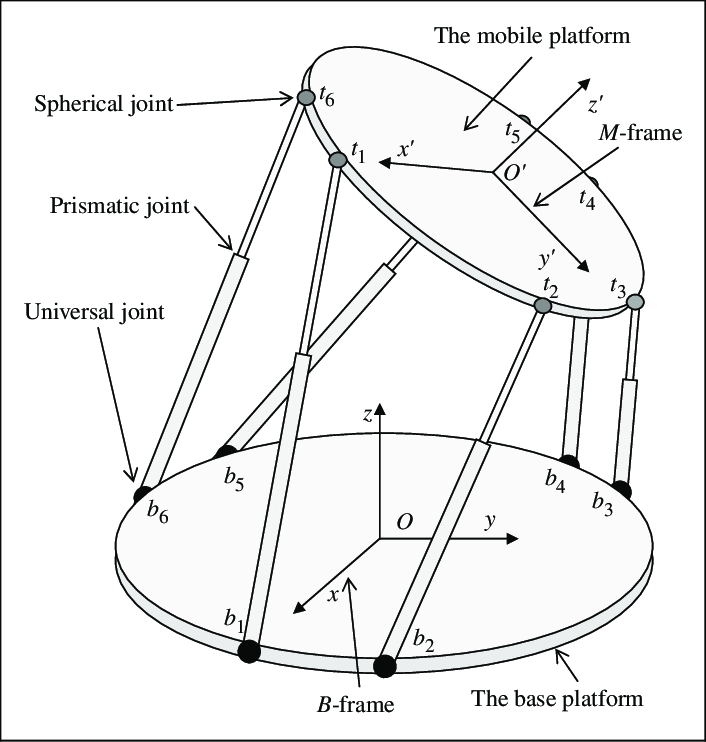
\includegraphics[width=0.5\linewidth]{stewart-platform.png}
    \caption{A Stewart Platform with 6 legs. Each leg connects to the base via a universal joint and to the top platform via a spherical joint, with a prismatic joint in between.}
    \label{fig:stewartplatform}
\end{figure}

Each leg connects to the base through a \textbf{universal joint} (2 DoF) and to the top plate through a \textbf{spherical joint} (3 DoF). The leg itself extends and retracts via a \textbf{prismatic joint} (1 DoF). That gives each leg 3 joints and $2 + 1 + 3 = 6$ total freedoms per leg.

Now let's count:
\begin{itemize}
    \item m = 6 (spatial mechanism)
    \item N = 14 (6 legs $\times$ 2 links per leg + base + top plate)
    \item J = 18 (6 legs $\times$ 3 joints per leg)
    \item $\sum_{i=1}^{J} f_i = 6 \times (2 + 1 + 3) = 36$
\end{itemize}

Plugging in:
\[
    \text{dof} = 6(14 - 1 - 18) + 36 = 6(-5) + 36 = -30 + 36 = 6
\]

The Stewart Platform has \textbf{6 degrees of freedom}: 3 translational and 3 rotational, giving the top plate full control over its position and orientation in space. There are limits to the range of motion, but range limits do not reduce the number of DoF.

\section{When Gr\"{u}bler's Formula Breaks}

Gr\"{u}bler's formula is powerful, but it can fail. The simplest example is a door mounted on two hinges. There are 2 links (the door and the wall, which serves as the ground), connected by 2 revolute joints (the hinges). Each hinge allows 1 freedom. This is a spatial mechanism, so $m = 6$. Gr\"{u}bler's gives:
\[
    \text{dof} = 6(2 - 1 - 2) + (1 + 1) = 6(-1) + 2 = -4
\]

Negative four degrees of freedom is nonsensical. The door clearly has 1 DoF: it swings open and shut. The problem is that both hinge axes are \textbf{collinear}. They lie on the same vertical line, so the second hinge removes no freedom that the first hasn't already removed. Its constraints are entirely redundant. The formula counts them anyway.

A subtler example is a planar mechanism with 3 equal length links (Figure~\ref{fig:planarmechanism}).

\begin{figure}[H]
    \centering
    \adjustbox{frame}{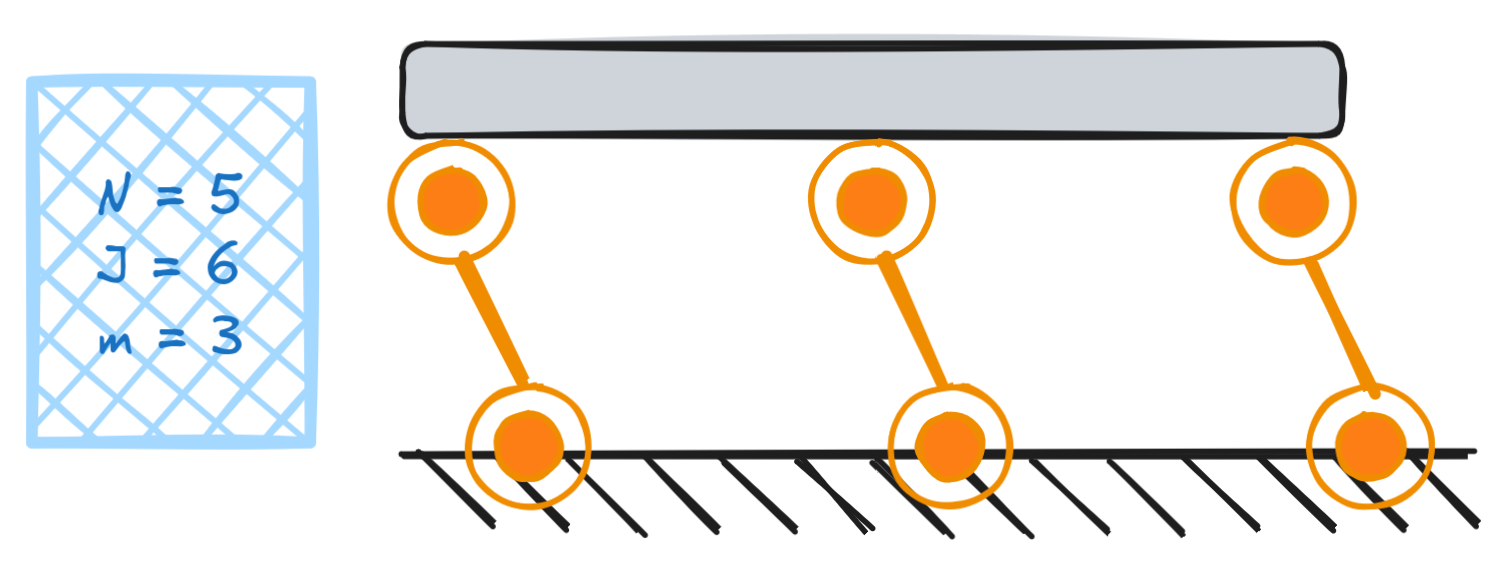
\includegraphics[width=0.5\linewidth]{planar-mechanism.png}}
    \caption{A planar parallel mechanism with 3 equal length links, each connected to the ground and to the top platform by a revolute joint (N = 5, J = 6, m = 3).}
    \label{fig:planarmechanism}
\end{figure}

Each link connects to the ground and to the top platform via a revolute joint. That gives N = 5, J = 6, m = 3, and every $f_i$ = 1. Gr\"{u}bler's predicts $\text{dof} = 3(5 - 1 - 6) + 6 = 0$. Yet, since the links are equal in length and the joints are symmetrically spaced, the top platform clearly moves. The formula can't see this because it's purely topological. It counts links and joints but knows nothing about the geometry. The symmetric layout makes some constraints redundant, and Gr\"{u}bler's has no way of detecting that. To catch these cases, you need to look at the actual constraint equations (typically through a Jacobian analysis) and check their rank.

In both cases, the root cause is the same: \textbf{the geometry of the mechanism makes some constraints redundant}, and Gr\"{u}bler's formula, being purely topological, cannot detect this.

\noindent\textit{I built an interactive walkthrough of Grübler's formula that lets you step through the three stages visually, explore different joint types, and see a case where the formula breaks down. Available at: \url{your-link-here}}


\section{What's Next}

I don't know. Though, I'm brushing up on some fundamentals while applying them in projects, because the best way to learn is to do (thanks Naval).

\end{document}
